\documentclass[a4paper,11pt]{article}

\usepackage[T1]{fontenc}
\usepackage[utf8]{inputenc}
\usepackage{graphicx}
\usepackage{xcolor}
\usepackage{tcolorbox}
\usepackage{sectsty}
\usepackage{enumitem}
\usepackage{circuitikz}
\renewcommand\familydefault{\sfdefault}
\usepackage{tgheros}
\usepackage{amsmath,amssymb,amsthm,textcomp}
\usepackage{enumitem}
\usepackage{multicol}
\usepackage{tikz}

\usepackage{geometry}
\geometry{left=25mm,right=25mm,%
bindingoffset=0mm, top=20mm,bottom=20mm}





\linespread{1.3}

\newcommand{\linia}{\rule{\linewidth}{0.5pt}}

% custom theorems if needed
\newtheoremstyle{mytheor}
    {1ex}{1ex}{\normalfont}{0pt}{\scshape}{.}{1ex}
    {{\thmname{#1 }}{\thmnumber{#2}}{\thmnote{ (#3)}}}

\theoremstyle{mytheor}
\newtheorem{defi}{Definition}

% my own titles
\makeatletter

\renewcommand{\maketitle}{
\colorbox{gray!20}{\framebox[\linewidth]{ \huge \textsc{\@title} } 
\lfoot{\@title}
}

}
\makeatother
%%%



% custom footers and headers
\usepackage{fancyhdr}
\pagestyle{fancy}
\lhead{}
\chead{Métodos Numéricos - 1C2020}
\rhead{}
\cfoot{}
\rfoot{Pagina \thepage}
\renewcommand{\footrulewidth}{0.2pt}
%


\renewcommand\headrulewidth{.5pt}
\makeatletter
\def\headrule{{\if@fancyplain\let\headrulewidth\plainheadrulewidth\fi
\hrule\@height\headrulewidth\@width\headwidth
\vskip 1pt% 2pt between lines
\hrule\@height1.5pt\@width\headwidth% lower line with .5pt line width
\vskip-\headrulewidth
\vskip-1.5pt}}
\makeatother


\makeatletter

\newcommand{\inlineitem}[1][]{%
\ifnum\enit@type=\tw@
    {\descriptionlabel{#1}}
  \hspace{\labelsep}
\else
  \ifnum\enit@type=\z@
       \refstepcounter{\@listctr}\fi
    \quad\@itemlabel\hspace{\labelsep}
\fi}
\makeatother




% code listing settings
\usepackage{listings}
\lstset{
    language=Python,
    basicstyle=\ttfamily\small,
    aboveskip={1.0\baselineskip},
    belowskip={1.0\baselineskip},
    columns=fixed,
    extendedchars=true,
    breaklines=true,
    tabsize=4,
    prebreak=\raisebox{0ex}[0ex][0ex]{\ensuremath{\hookleftarrow}},
    frame=lines,
    showtabs=false,
    showspaces=false,
    showstringspaces=false,
    keywordstyle=\color[rgb]{0.627,0.126,0.941},
    commentstyle=\color[rgb]{0.133,0.545,0.133},
    stringstyle=\color[rgb]{01,0,0},
    numbers=left,
    numberstyle=\small,
    stepnumber=1,
    numbersep=10pt,
    captionpos=t,
    escapeinside={\%*}{*)}
}

%%%----------%%%----------%%%----------%%%----------%%%

\begin{document}


\title{Trabajo práctico 4}

\author{Ulises Bussi-Javier Portillo, Universidad Nacional de Quilmes}


\maketitle \vspace{20pt}



\section*{Ecuaciones Diferenciales}

\subsection*{Ejercicio 1}
La ley de Gravitación Universal de Newton, es la primera expresión que relaciona las propiedades físicas de dos cuerpos celestes con la fuerza mutua que se ejercen.  Esta ley es expresada con la siguiente ecuación:

\begin{equation*}
  \vec F = -G \frac{m_1 * m_2}{|\vec r|^2} \hat r
\end{equation*}

Donde $G=6.67\times10^{-11} \frac{N m^2}{{kg}^2} $ es conocida como la constante de gravitación universal de Newton, $m_1$ y $m_2$ son las masas de los cuerpos celestes, $\vec r$ es el vector que une ambos cuerpos ($\vec r = [x,y]$,el modulo del vector es $|\vec r|$ y el versor es $\hat r$ vector de largo 1).

\begin{figure}[h]
\centering
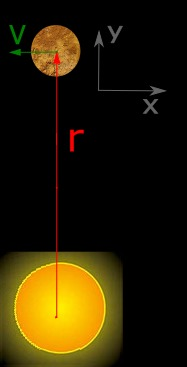
\includegraphics[width=.3\linewidth]{f1_p.jpeg}
\label{fig:f1}
\caption{Esquema de planetas y sistema de referencia.}

\end{figure}


Si consideramos un cuerpo celeste de masa $m_1$ que gira alrededor del sol (de masa $m_2 = 1.98\times10^{30}kg$ ubicado como se ve en la figura \ref{fig:f1} en $[1.495e11 , 0]m$  y una velocidad $[0 ,-2.977e4]m/s$, podemos escribir la segunda ley de Newton para el cuerpo:

\begin{equation*}
\vec F = m \vec a
\end{equation*}

Donde $\vec a =\vec r''$ (como vectores $[a_x,a_y]= [x'',y'']$) .


La combinación de estas ecuaciones lleva a una ecuación diferencial.
\begin{enumerate}
\item Plantee la ecuación diferencial. 
\item Transforme a variables de estado para llevarlo a un sistema de ecuaciones diferenciales de orden 1. Exprese este sistema de ecuaciones diferenciales.
\item Resuelva la ecuación diferencial utilizando el método de Euler con paso $h= 24h$ para el periodo equivalente a 1000 pasos *.
\item Resuelva la ecuación diferencial utilizando el método de Heun con paso $h= 24h$ para el periodo equivalente a 1000 pasos *.
\item Es posible lograr, en este problema,que el método de Euler que la conseguida la calidad del métodoHeun? Que sucedería si el tiempo se va a infinito?
\end{enumerate}

* Para ambos casos grafique la trayectoria ($x$ vs $y$), explique que sucede, de una interpretación.

\subsection*{Ejercicio 2}

El pais se encuentra en medio de una pandemia. Luego de su gran desempeño en la materia de Métodos Númericos, el presidente de la Nación lo asigna como asesor técnico del ministro de salud. Su tarea es revisar los códigos en Matlab que el propio ministro desarrolló.

El ministro de salud le comenta que, para simular la propagación del virus, usó un modelo tipo SIR (SIR.m) obteniendo el gráfico que se observa a continuación:

\begin{figure}[h]
\centering
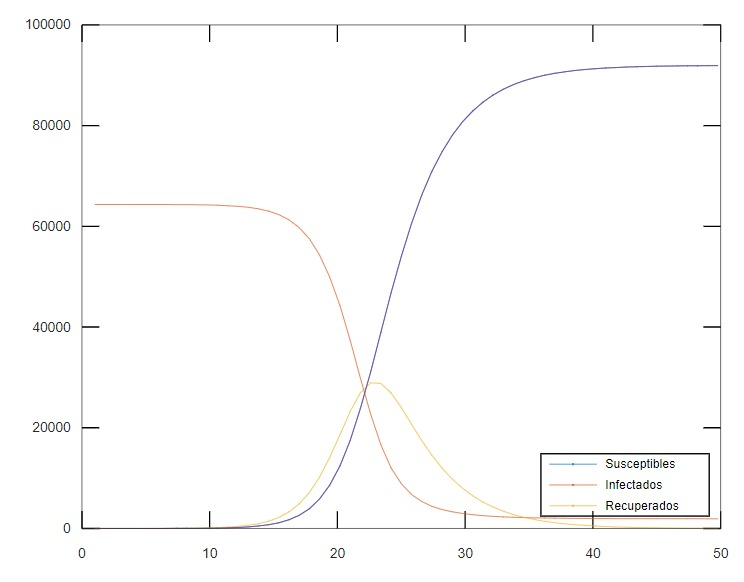
\includegraphics[width=.85\linewidth]{prediccion.jpeg}
\label{fig:f2}
\caption{Esquema de planetas y sistema de referencia.}

\end{figure}

El ministro expresó su preocupación, comentandole que la predicción la hizo para su ciudad natal (Gerli), y que según su estimación, en el pico iban a existir 29000 infectados. Usted comienza a analizar la información:


\begin{enumerate}
\item En la imagen enviada por el ministro hay algo totalmente incoherente, ¿Que es? Explique. (De ser necesario, busque información a cerca del modelo SIR. No es necesario que entienda el modelo en profundidad, pero si, al menos, que entienda que significan sus siglas y pueda interpretar el gráfico.)

\item Según el modelo utilizado por el ministro, ¿Cuántos infectados habrá en el pico de la pandemia?

\item Modificando el código, intente solucionar el problema encontrado en el item anterior. (Pista: los parametros $beta$ y $gamma$ fueron determinados con precisión, yo que usted, no los modificaría). 

\item Vuelva a calcular el número de infectados en el pico (con el código corregido).

\item Aumentando en un 20\% el parámetro beta. ¿Cómo cambia la curva con este aumentó en beta?

\end{enumerate}
\end{document}